% GNUPLOT: LaTeX picture with Postscript
\begingroup
  \makeatletter
  \providecommand\color[2][]{%
    \GenericError{(gnuplot) \space\space\space\@spaces}{%
      Package color not loaded in conjunction with
      terminal option `colourtext'%
    }{See the gnuplot documentation for explanation.%
    }{Either use 'blacktext' in gnuplot or load the package
      color.sty in LaTeX.}%
    \renewcommand\color[2][]{}%
  }%
  \providecommand\includegraphics[2][]{%
    \GenericError{(gnuplot) \space\space\space\@spaces}{%
      Package graphicx or graphics not loaded%
    }{See the gnuplot documentation for explanation.%
    }{The gnuplot epslatex terminal needs graphicx.sty or graphics.sty.}%
    \renewcommand\includegraphics[2][]{}%
  }%
  \providecommand\rotatebox[2]{#2}%
  \@ifundefined{ifGPcolor}{%
    \newif\ifGPcolor
    \GPcolorfalse
  }{}%
  \@ifundefined{ifGPblacktext}{%
    \newif\ifGPblacktext
    \GPblacktexttrue
  }{}%
  % define a \g@addto@macro without @ in the name:
  \let\gplgaddtomacro\g@addto@macro
  % define empty templates for all commands taking text:
  \gdef\gplbacktext{}%
  \gdef\gplfronttext{}%
  \makeatother
  \ifGPblacktext
    % no textcolor at all
    \def\colorrgb#1{}%
    \def\colorgray#1{}%
  \else
    % gray or color?
    \ifGPcolor
      \def\colorrgb#1{\color[rgb]{#1}}%
      \def\colorgray#1{\color[gray]{#1}}%
      \expandafter\def\csname LTw\endcsname{\color{white}}%
      \expandafter\def\csname LTb\endcsname{\color{black}}%
      \expandafter\def\csname LTa\endcsname{\color{black}}%
      \expandafter\def\csname LT0\endcsname{\color[rgb]{1,0,0}}%
      \expandafter\def\csname LT1\endcsname{\color[rgb]{0,1,0}}%
      \expandafter\def\csname LT2\endcsname{\color[rgb]{0,0,1}}%
      \expandafter\def\csname LT3\endcsname{\color[rgb]{1,0,1}}%
      \expandafter\def\csname LT4\endcsname{\color[rgb]{0,1,1}}%
      \expandafter\def\csname LT5\endcsname{\color[rgb]{1,1,0}}%
      \expandafter\def\csname LT6\endcsname{\color[rgb]{0,0,0}}%
      \expandafter\def\csname LT7\endcsname{\color[rgb]{1,0.3,0}}%
      \expandafter\def\csname LT8\endcsname{\color[rgb]{0.5,0.5,0.5}}%
    \else
      % gray
      \def\colorrgb#1{\color{black}}%
      \def\colorgray#1{\color[gray]{#1}}%
      \expandafter\def\csname LTw\endcsname{\color{white}}%
      \expandafter\def\csname LTb\endcsname{\color{black}}%
      \expandafter\def\csname LTa\endcsname{\color{black}}%
      \expandafter\def\csname LT0\endcsname{\color{black}}%
      \expandafter\def\csname LT1\endcsname{\color{black}}%
      \expandafter\def\csname LT2\endcsname{\color{black}}%
      \expandafter\def\csname LT3\endcsname{\color{black}}%
      \expandafter\def\csname LT4\endcsname{\color{black}}%
      \expandafter\def\csname LT5\endcsname{\color{black}}%
      \expandafter\def\csname LT6\endcsname{\color{black}}%
      \expandafter\def\csname LT7\endcsname{\color{black}}%
      \expandafter\def\csname LT8\endcsname{\color{black}}%
    \fi
  \fi
  \setlength{\unitlength}{0.0500bp}%
  \begin{picture}(9118.00,4320.00)%
    \gplgaddtomacro\gplbacktext{%
      \colorrgb{0.00,0.00,0.00}%
      \put(740,640){\makebox(0,0)[r]{\strut{}90}}%
      \colorrgb{0.00,0.00,0.00}%
      \put(740,1500){\makebox(0,0)[r]{\strut{}95}}%
      \colorrgb{0.00,0.00,0.00}%
      \put(740,2360){\makebox(0,0)[r]{\strut{}100}}%
      \colorrgb{0.00,0.00,0.00}%
      \put(740,3219){\makebox(0,0)[r]{\strut{}105}}%
      \colorrgb{0.00,0.00,0.00}%
      \put(740,4079){\makebox(0,0)[r]{\strut{}110}}%
      \colorrgb{0.00,0.00,0.00}%
      \put(860,440){\makebox(0,0){\strut{}$(1, *, *)$}}%
      \colorrgb{0.00,0.00,0.00}%
      \put(1945,440){\makebox(0,0){\strut{}$(2, *, *)$}}%
      \colorrgb{0.00,0.00,0.00}%
      \put(3031,440){\makebox(0,0){\strut{}$(3, *, *)$}}%
      \colorrgb{0.00,0.00,0.00}%
      \put(4116,440){\makebox(0,0){\strut{}$(4, *, *)$}}%
      \colorrgb{0.00,0.00,0.00}%
      \put(5202,440){\makebox(0,0){\strut{}$(5, *, *)$}}%
      \colorrgb{0.00,0.00,0.00}%
      \put(6287,440){\makebox(0,0){\strut{}$(6, *, *)$}}%
      \colorrgb{0.00,0.00,0.00}%
      \put(7373,440){\makebox(0,0){\strut{}$(7, *, *)$}}%
      \colorrgb{0.00,0.00,0.00}%
      \put(8458,440){\makebox(0,0){\strut{}$(8, *, *)$}}%
      \colorrgb{0.00,0.00,0.00}%
      \put(160,2359){\rotatebox{90}{\makebox(0,0){\strut{}Tiempo de ejecuci\'on (ticks)}}}%
      \colorrgb{0.00,0.00,0.00}%
      \put(4659,140){\makebox(0,0){\strut{}Quantums por core}}%
    }%
    \gplgaddtomacro\gplfronttext{%
      \csname LTb\endcsname%
      \put(7555,3916){\makebox(0,0)[r]{\strut{}M\'inimo}}%
      \csname LTb\endcsname%
      \put(7555,3716){\makebox(0,0)[r]{\strut{}M\'aximo}}%
    }%
    \gplbacktext
    \put(0,0){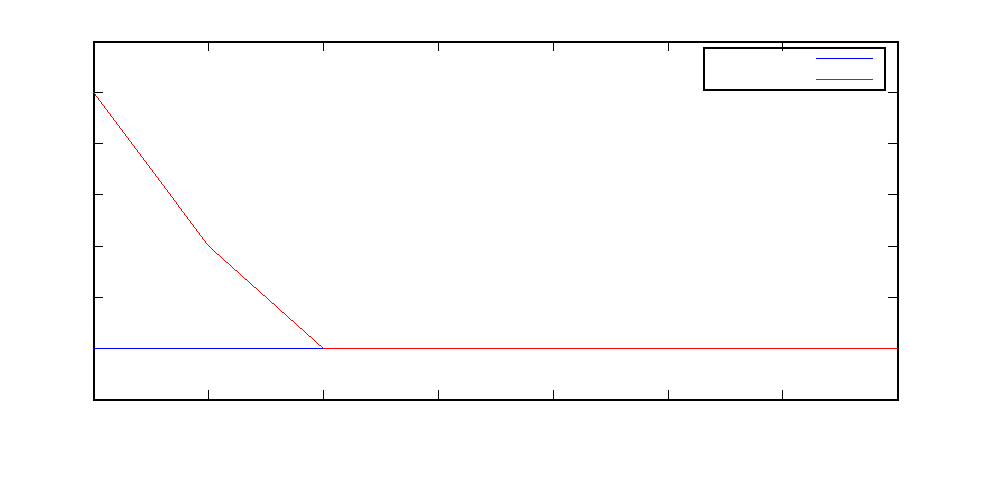
\includegraphics{ej7-grafico-runtime-3-cores}}%
    \gplfronttext
  \end{picture}%
\endgroup
